% rubber: set program xelatex
\documentclass[a4paper,12pt]{article}

\usepackage{xltxtra}
\usepackage{amsmath,amsthm,amssymb}
\usepackage{mathtools}

\usepackage[autostyle=true]{csquotes}
\usepackage{polyglossia}
\setmainlanguage{english}

% Fonts
\setmainfont{CMU Serif}
\setsansfont{CMU Sans Serif}
\setmonofont{CMU Typewriter Text}
\usepackage[xetex, colorlinks=true, citecolor=blue, linkcolor=blue]{hyperref}

\usepackage{fancyhdr} 
\pagestyle{fancy}

\usepackage{graphicx}
\usepackage{subfigure} 
\usepackage{float} 
\usepackage{siunitx}

% Source code listings
\usepackage{listings}
\usepackage{color}
\usepackage{matlab-prettifier}
\lstdefinestyle{My-Matlab}
{
  style               = MatlabBaseStyle@mlpr,
  basicstyle          = \color{black}\ttfamily\small, 
  mllastelementstyle  = \color{black}                    ,
  mlkeywordstyle      = \color[RGB]{000,000,255}         ,
  mlcommentstyle      = \color[RGB]{034,139,034}         ,
  mlstringstyle       = \color[RGB]{160,032,240}         ,
  mlsyscomstyle       = \color[RGB]{178,140,000}         ,
  mlsectiontitlestyle = \commentStyle@mlpr      \bfseries,
  mlsharedvarstyle    = \color[RGB]{000,163,163}         ,
  mlplaceholderstyle  = \mleditorphstyle,
}


% Commands
\newcommand{\HRule}{\rule{\linewidth}{0.5mm}}

\begin{document}

\begin{minipage}{0.50\textwidth} 
	\begin{flushleft}
	
\includegraphics[scale = 0.50]{Images/Logo-vibot.png}
	\end{flushleft}
\end{minipage}
\begin{minipage}{0.50\textwidth} 
	\begin{flushright}
		
\includegraphics[scale = 0.50]{Images/Logo-ub.png}
	\end{flushright}
\end{minipage}

\begin{center} 
	\vspace*{-1cm}
	\textsc{\Large University of Burgundy}\\[0.5cm]

	\textsc{\Large Masters in Computer Vision}
\end{center}
\vspace*{-0.5cm}
\HRule
\vspace*{4cm}


\begin{minipage}{0.9\textwidth} 
	\begin{center}																					%%%
		\textsc{\LARGE MSFT Module - SFM + IMU} \\[0.5cm]
		\textsc{\LARGE \textbf{Report on 4 Points vs 2+1 Points Algorithms}} \\
		
	\end{center}
\end{minipage}\\[1.5cm]

\begin{center}
{ \Large 
	by \\[0.25cm]
	\textbf{Tsagkatakis Ioannis} \\[1.5cm]
	Under the supervision of \\[0.25cm]
	\textbf{Dr. Cédric Demonceaux} \\
}
\end{center}

\vspace*{2cm}

\begin{center}
	\today
\end{center}
% End First page
\newpage

\section{Introduction}

When we are estimating the homography, at least 8 points are needed, because after after normalization the 9 components of
the essential matrix is reduced to 8. But if we know some prior information about the motion of the camera like rotations and 
angles we can decrease the number of points required. In this project i compare the classical linear 4 points algorithm and the
linear 2 points, assumming that the vertical direction of the camera is known.

\section{The 4 points algorith} 
When all the points belongs to the same plane, then we need only 4 point. The homography can be computing using the equation\eqref{eq:eq1}

\begin{equation}
	\mathbf{H} = \mathbf{R} - \frac{\mathbf{t} \ast \mathbf{N}^T }{d}
	\label{eq:eq1}
\end{equation}
where, $\mathbf{H}$ the  Homography, 
 $\mathbf{R}$, the rotation between two camera views,
$\mathbf{t}$ the translation between two camera views,
$\mathbf{N}$ the normal vector of the plane of points and
$d$ the distance between the plane and the camera.\\[8pt]

The points $\mathbf{p}$ and $\mathbf{p}'$ are colinear so $\mathbf{p} \cong \mathbf{p}'$ and 
\begin{equation}
	\mathbf{p}' \times \mathbf{H} \mathbf{p} = \mathbf{0}
	\label{eq:eq2}
\end{equation}

\noindent The second equation equation\eqref{eq:eq2} can be used for the verification of the computed Homography.

\subsection{Matlab code and results}
First $50$ are randomly generated  in a plane of equation
$\mathbf{N}^T \mathbf{X}_w +d = 0$ in the world frame $(O_w , X_w , Y_w , Z_w )$. The camera is calibrated
with the rotation $R_i$ and $T_i$ of the world coordinate $(X_w = R_i X_{ci} + T_i )$ and  $\mathbf{N} = \left[0,0,1\right]$. The points are shown in figure~\ref{fig:points}.

\begin{figure}[tb]
         \centering
         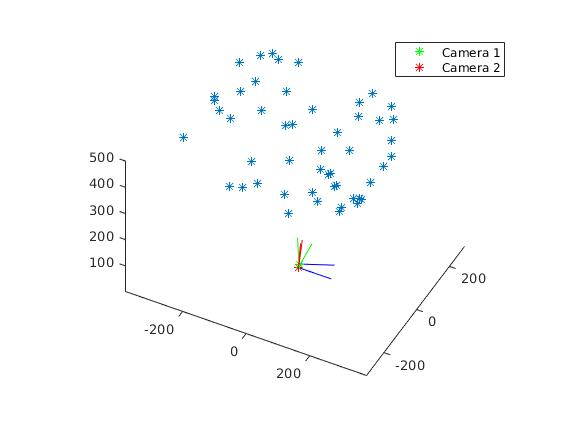
\includegraphics[width=8cm]{Images/points3D.png}
         \caption{50 random points located on a plane}
 	\label{fig:points}
\end{figure}

\vspace*{8pt}
\noindent The Theoretical Homography $\mathbf{H}$ is calculated 
\begin{lstlisting}[style=My-Matlab]
N = [0,0,1]';
d = (N'*T1-zposition); 
\end{lstlisting}
Where \texttt{d} is the distnace between the 3D points located \texttt{zposition} away from the  ground plane and the 1st camera. We multiply by the  \texttt{norm(N)}  of the ground plane and  and the translation \texttt{T1} of camera 1, to get the distance from where the 1st camera is 
 moved in z-direction and then subtract the \texttt{zposition} from it.

\begin{verbatim}
### TEST 0 ##
The Theoretical Homography

H =

    0.8896   -0.4121    0.0270
    0.4111    0.8907    0.0190
   -0.0313    0.0046    1.0000

Estimated Homography (4 Point Algorithm)

H4pt =

    0.8896   -0.4121    0.0270
    0.4111    0.8907    0.0190
   -0.0313    0.0046    1.0000

  
\end{verbatim}


\section{The 2 points Algorithm}
If the points are on the same plane, and this plane is vertical, then the 4 points can
then be reduced to just 2 points. Then the homography is given by equation \eqref{eq:eq3}

\begin{equation}
	H = R_y + [t_x,t_y,t_t]^T [n_x,0,n_z]
	\label{eq:eq3}
\end{equation}


\noindent The \eqref{eq:eq3} is exapnded in only 4 equations and the system is underdetermined. By using SVD:

\begin{align}
	A h &= b \\
	A &= U D V^T \\
	h &= Vy +w \upsilon \\
	\upsilon &= U^Tb / D
	\label{eq:eq4}
\end{align}
where $\upsilon$ is the last column of vector $V$ and from $\left| H^T H - \mathbf{I}\right| = 0$ we get $w$ as the solution of a 4th order polynomial.

\begin{verbatim}
Theoretical Homography (2 angles known)

HV2 =

    0.9063   -0.4226    0.0007
    0.4226    0.9063    0.0083
         0         0    1.0208

Verification of theoretical Homography (2 angles known)

ans =

    0.2219
    0.1330
    0.9660


GroundTruth =

    0.2219
    0.1330
    0.9660

Estimated Homography (2+1 Point Algorithm)

EstimatedH =

    0.8878   -0.4140    0.0007
    0.4140    0.8878    0.0081
         0         0    1.0000

Verification of Yaw Angle

Yaw =

    0.4363


YawGroundTruth =

    0.4363

calculated and Theoretical translational vector

T2E =

   -0.0324
   -0.3700
   -0.9285


T2t =

    0.3486
    3.9848
   10.0000
             
\end{verbatim}

\subsection{Conclusions}
The results is the same as expected and our caluclations are correct.

\section{Matlab Tests}
\subsection{Test1}
Example with different datas, propose a test with different positions of the
second camera $(R1 = I, T1 = 0)$ with angles of rotation between $\ang{0}$ and $\qng{45}$ and
translation of 0 to 100. The points are shown in figure~\ref{fig:points-t1}.

\begin{figure}[tb]
         \centering
         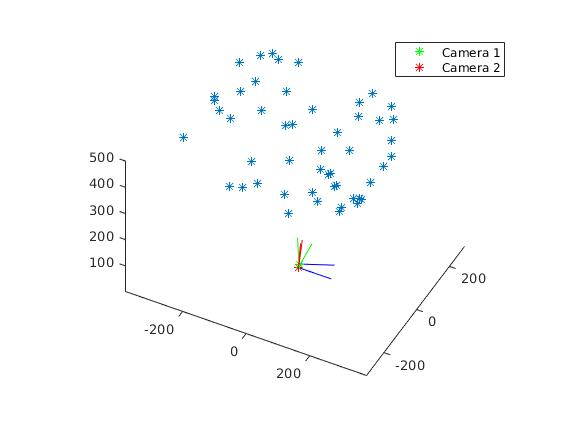
\includegraphics[width=8cm]{Images/points3D.png}
         \caption{Test1 different data}
 	\label{fig:points-t1}
\end{figure}

\subsubsection{The 4 points algorithm}
\begin{verbatim}
### TEST 1 ##
The Theoretical Homography

The Theoretical Homography

H =

    1.4215    0.2506   -1.4480
    0.7545    1.5987    0.9532
    1.2558   -1.2442    1.0000

Estimated Homography (4 Point Algorithm)

H4pt =

    1.4215    0.2506   -1.4480
    0.7545    1.5987    0.9532
    1.2558   -1.2442    1.0000
\end{verbatim}
The results is the same as expected.

\subsubsection{The 2 points algorithm}

Theoretical Homography (2 angles known)

\begin{verbatim}
### TEST 1 ##
Theoretical Homography (2 angles known)

HV2 =

    0.9848    0.1736   -0.0232
   -0.1736    0.9848   -0.0162
         0         0    0.9800

True Theoretical Homography (2 angles known)

TrueHomography =

    1.0049    0.1772   -0.0236
   -0.1772    1.0049   -0.0166
         0         0    1.0000

Estimated Homography (2+1 Point Algorithm)

EstimatedH =

    1.0049    0.1772   -0.0236
   -0.1772    1.0049   -0.0166
\end{verbatim}
The results is the same as expected.

\subsection{Test2}
Example with noise, propose a test with different camera positions $(R1 =
I, T1 = 0)$ with angles of rotation between $\rad{0}$ and $\rad{45}$ and translation of 0 to
100 AND white noise in image points of camera 2 between 0 to 1 pixel std (use
RANSAC functions).

The camera location and the points are shown in figure~\ref{fig:points2}. Because with 4-Point Algorithm, the solution of AE = 0 is a
 2-dimentional space, so we will take only x and y in our  case.

\begin{figure}[tb]
         \centering
         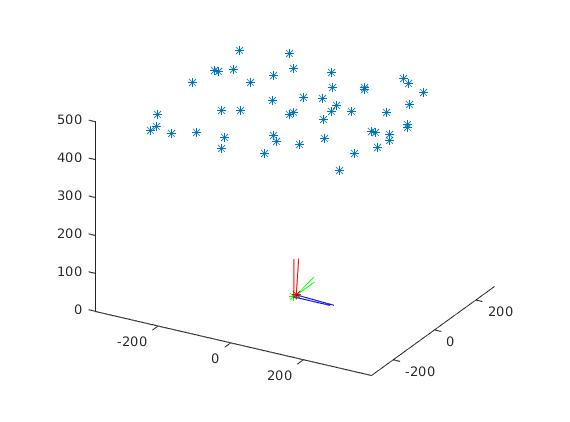
\includegraphics[width=8cm]{Images/points3D-test2.jpg}
         \caption{Test points with noise  and cameras for test 2}
 	\label{fig:points2}
\end{figure}

\subsubsection{The 4 points algorithm}
\begin{verbatim}
### TEST 2 ##
The Theoretical Homography

H =

    1.1010    0.2950   -0.9308
   -0.0459    1.4353    0.4211
    0.9999   -0.2590    1.0000

Estimated Homography (4 Point Algorithm)

H4ptS =

    1.1010    0.2950   -0.9308
   -0.0459    1.4353    0.4211
    0.9999   -0.2590    1.0000

Estimated Homography (4 Point RANSAC Algorithm)

H4pt =

    1.1010    0.2950   -0.9308
   -0.0459    1.4353    0.4211
    0.9999   -0.2590    1.0000

Errors using Ransac

diff =

   444.0892e-018   610.6227e-018  -333.0669e-018
  -215.1057e-018  -222.0446e-018   166.5335e-018
  -444.0892e-018   388.5781e-018     0.0000e+000

Error(SSD) in 4 point estimation, with noise is : 1.1525e-30
\end{verbatim}


\subsubsection{The 2 points algorithm}

Theoretical Homography (2 angles known)

\begin{verbatim}
### TEST 2 ##
Theoretical Homography (2 angles known)

HV2 =

    0.9659    0.2588   -0.0110
   -0.2588    0.9659    0.0361
         0         0    0.9600

True Theoretical Homography (2 angles known)

TrueHomography =

    1.0062    0.2696   -0.0115
   -0.2696    1.0062    0.0376
         0         0    1.0000

Estimated Homography (2+1 Point Algorithm RANSAC)

EstimatedH =

    1.1010    0.2950   -0.9308
   -0.0459    1.4353    0.4211
    0.9999   -0.2590    1.0000

Estimated Homography (2+1 Point Algorithm No RANSAC)

EstimatedH2 =

    1.0062    0.2696   -0.0115
   -0.2696    1.0062    0.0376
         0         0    1.0000

Errors using Ransac

diff =

   -94.8593e-003   -25.4175e-003   919.2915e-003
  -223.6908e-003  -429.1107e-003  -383.5226e-003
  -999.8786e-003   258.9614e-003     0.0000e+000

Error(SSD) in 2 point estimation, with noise is : 2.3028
\end{verbatim}

\subsubsection{Conclusions}
Due to noise we get different results as expected. Both results obtained from RANSAC algorithm are 
approching the ground truth and the difference has minimized. Most outliers are removed and we dont get exactly thes smae results.


\subsection{Test3}
Example with noise on IMU informations, propose a test with different camera positions $(R1 =
I, T1 = 0)$ with angles of rotation between $\rad{0}$ and $\rad{45}$ and translation of 0 to
100 AND white noise in image points of camera 2 between 0 to 1 pixel std AND white noise in IMU between $\rad{0}$ and $\rad{2}$ (use
RANSAC functions).

The camera location and the points are shown in figure~\ref{fig:points3}. 

\begin{figure}[tb]
         \centering
         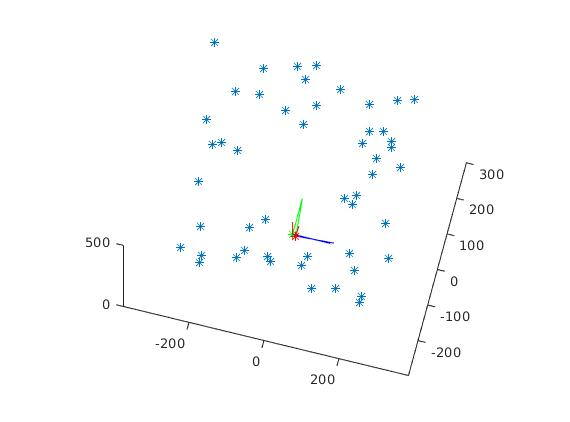
\includegraphics[width=8cm]{Images/points3D-test3.jpg}
         \caption{Test points with noise and noise in IMU for test 3}
 	\label{fig:points3}
\end{figure}
\subsubsection{The 4 points algorithm}
\begin{verbatim}
### TEST 3 ##
The Theoretical Homography

H =

    1.0201    0.0952   -0.1095
   -0.0905    1.0231    0.0690
    0.0968   -0.0475    1.0000

Estimated Homography (4 Point Algorithm)

H4pt =

    1.0195    0.0951   -0.1089
   -0.0903    1.0226    0.0695
    0.0971   -0.0470    1.0000

Error(SSD) in 4 point estimation, with noise is : 1.5969e-06
\end{verbatim}


\subsubsection{The 2 points algorithm}

Theoretical Homography (2 angles known)

\begin{verbatim}
### TEST 3 ##
Theoretical Homography (2 angles known)

HV2 =

    0.9957    0.0930   -0.0188
   -0.0930    0.9957    0.0138
         0         0    0.9800

True Theoretical Homography (2 angles known)

TrueHomography =

    1.0160    0.0949   -0.0192
   -0.0949    1.0160    0.0141
         0         0    1.0000

Estimated Homography (2+1 Point Algorithm)

EstimatedH =

    1.0201    0.0952   -0.1095
   -0.0905    1.0231    0.0690
    0.0968   -0.0475    1.0000

Error(SSD) in 2 point estimation, with noise is : 0.02289
\end{verbatim}

\section{Conclusion}
In this practical work, we test the 4 pts and 2 pts algorithms for the scenario
of points on the plane and on the vertical plane respectively. Then the
algorithms are tested with noisy points and noisy IMU information. The
estimated results are approaching the ground truth.

The code of this project is on Github repository \url{https://github.com/jtsagata/IMULab}.

\clearpage
\end{document} % NOTHING AFTER THIS LINE IS PART OF THE DOCUMENT
